
 In the case of uniform point distributions, we could obtain precise estimates for the threshold $n^*$ and use it to 
 choose between the truncation and expansion algorithms to achieve optimal complexity. However, when the source and 
 target distributions are highly non-uniform, as is the case in most practical applications, it is not as
 straightforward. Note that the expansion algorithm is advantageous when there are many sources within a FGT box and
 the truncation algorithm is more suitable otherwise. Hence, to achieve optimal complexity in the non-uniform case, we 
 need a hybrid algorithm that uses the expansion algorithm in regions with a high density of points and the 
 truncation algorithm in other regions. We use an {\em octree} \cite{clr90} data structure to efficiently
 separate out regions with a dense point distribution from regions with a sparse point distribution and use
 it to appropriately choose between the truncation and expansion algorithm in each region. A similar idea was
 used in \cite{veerapaneni08}.  
 
{\em Primer on octrees.} An octree is a tree data structure that is used for spatial decomposition. Every
node of an octree has a maximum of eight children. An octant with no children is
called a ``{\em leaf}'' and an octant with one or more children is
called an ``{\em interior octant}''. The only octant with no parent is the
 ``{\em root}'' and all other octants have exactly one parent. The depth of an octant 
 from the root is referred to as its ``{\em level}''. We use a ``{\em linear}'' octree
representation (i.e., we exclude interior octants) using the ``{\em
Morton encoding}'' scheme \cite{morton66}. Any octant in the domain can be uniquely
identified by specifying one of its vertices, also known as its ``{\em
anchor}'', and its level in the tree. By convention, the anchor of an
octant is its front lower left corner. 

\subsection{Octree based FGT algorithm}
\label{sc:octreefgt}

 Given a point distribution, we construct a linear octree such that there are no more than $m$ points contained within each leaf; we
 use the algorithm described in \cite{octPaper08} to do this. Note that regions with sparse point distributions will contain 
 leaves that are large in size and regions with dense point distributions will contain leaves that are small in size. Just as in 
 the uniform case, we partition the domain into FGT boxes of size $h = \sqrt{\delta}$. We denote the size of leaf $\ell$ by $|\ell|$.
 We use a heuristic parameter, $c$, to mark leaves as either ``Expand'' or ``Direct'' as follows (Figure \ref{f:directExpand}):

{\tt
\begin{algorithmic}
\STATE
  \FOR {each leaf $\ell$}
      \IF {$|\ell| > c h$}
          \STATE Mark $\ell$ as ``Direct''. 
      \ELSE
          \STATE Mark $\ell$ as ``Expand''. 
      \ENDIF
  \ENDFOR
\STATE
\end{algorithmic}
}

\begin{figure}
\begin{center}
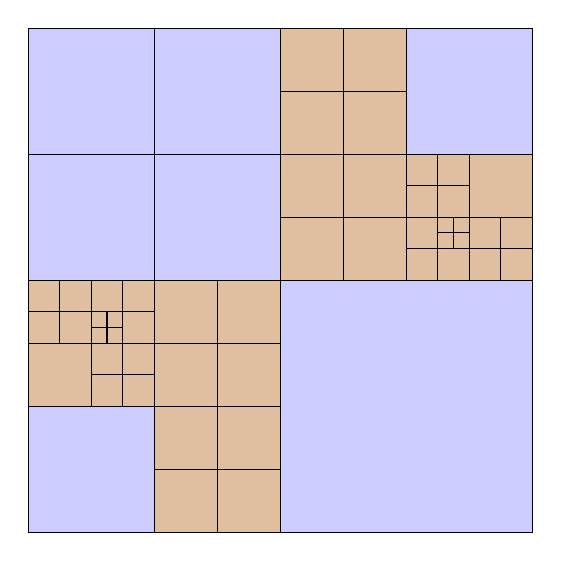
\begin{tikzpicture}[scale=0.4]

\draw[fill=blue!20] (0,8) rectangle +(8,8);
\draw[fill=blue!20] (8,0) rectangle +(8,8);
\draw[fill=blue!20] (0,0) rectangle +(4,4);
\draw[fill=blue!20] (12,12) rectangle +(4,4);

\draw[fill=brown!50] (4,0) rectangle +(4,4);
\draw[fill=brown!50] (0,4) rectangle +(4,4);
\draw[fill=brown!50] (4,4) rectangle +(4,4);
\draw[fill=brown!50] (8,8) rectangle +(4,4);
\draw[fill=brown!50] (8,12) rectangle +(4,4);
\draw[fill=brown!50] (12,8) rectangle +(4,4);

%Draw the initial octree
\draw[step = 8] (0,0) grid (16,16);
\draw[step = 4] (8,8) grid(16,16);
\draw[step = 4] (0,8) grid(8,16);
\draw[step = 2] (0,4) grid(4,8);
\draw[step = 2] (4,4) grid (8,8);
\draw[step = 2] (4,0) grid (8,4);
\draw[step = 1] (2,4) grid (4,8);    	
\draw[step = 1] (0,6) grid (2,8);
\draw[step = 0.5] (2,6) grid (3,7);

\draw[step = 2] (8,8) grid(12,16);
\draw[step = 2] (12,8) grid (16,12);
    	    	
\draw[step = 1] (12,8) grid (14,12);
\draw[step = 1] (14,8) grid (16,10);
\draw[step = 0.5] (13,9) grid (14,10);    	    	    	    	
    	    	    	    	
\end{tikzpicture}
\caption{\label{f:directExpand} An example of a tree whose leaf nodes are distinguished based 
on their size. The ``large'' leaf nodes shown in brown color belong to $T_d$ and 
the ``small'' leaf nodes shown in blue color belong to $T_e$.}  
\end{center}
\end{figure}

We denote the set of direct leaves by $T_d$ and use $T_e$ to represent the set of expand leaves. Next,
we describe the sequence of steps involved in this algorithm.

[Add More Motivation here -- Shravan todo] 

\begin{description}
\item[\textbf{S2W}] In this step, we form the plane-wave expansions (\ref{eqn:s2w}) at all the boxes by visiting 
every leaf node in $T_e$. A particular leaf node $\ell$ can either be contained within a box $B$ or can enclose multiple number of boxes\footnote{Since the box size is chosen as $\sqrt{\delta}$, in the general case, there could be cases where boxes and leaf nodes overlap partially. Here, we make a simplifying assumption that $\delta = 2^{-n}$ for some positive 
integer $n$. This assumption can be relaxed easily by setting the box size to be $2^{\lfloor \log_2 \sqrt{\delta} \rfloor}$ correspondinlgy modifying the error estimates for FGT.}. In the former case, we add the contributions from all sources
within $\ell$ to the plane-wave expansion at $B$. In the latter case, we visit each constituent box $B$ and form 
its plane-wave expansion using only those sources that are contained in $B$.

\item[\textbf{W2D}] Initialize the transform at all targets within some direct leaf to zero. For
 each target, $x$, within some direct leaf, find all FGT boxes, $B$, such that $\mathcal{I}[B]$ contains $x$ and
 add the contributions from the respective plane-wave expansion, $w_k$ to the transform at the target as: 

\beq F(x) \, +=\, \sum_{|k| \leq p} \hat{G}(k)  w_k e^{i \lambda k \cdot (x - c^B)} \label{eqn:w2d} \eeq

Note, that for any FGT box, $B$, which is contained within some direct leaf the corresponding $w_k$ is zero.

\item[\textbf{D2D}] For each source $y \in T_d$, find all targets $x \in T_d$ such that $x \in \mathcal{I}[y]$ and
 modify the transform at $x$ as:
  
\beq F(x) \,+=\, G_\delta(\norm{x - y}) f(y) \label{eqn:d2d} \eeq

We make use of a few properties of the Morton ordering to efficiently search for all targets $x \in T_d \cap \mathcal{I}[y]$. These
are listed below:
\begin{enumerate}
\item Let $r = \sqrt{\delta \ln (\frac{1}{\epsilon})}$, $y_{min} = y - (r, r, r)$ and $y_{max} = y + (r, r, r)$. Then, the Morton id of
any point in $\mathcal{I}[y]$ will be $\geq$ that of $y_{min}$ and will be $\leq$ that of $y_{max}$.
\item If a point, $z$, is contained within a leaf, $\ell$, then the Morton id of $z$ will be greater than that of $\ell$.
\item If the Morton id of a leaf $l_1$ is less than that of another leaf $l_2$, then the Morton id of any point, $z$, which is
 contained within $l_1$ will also be lesser than that of $l_2$.
\end{enumerate}

\item[\textbf{W2L}] Only the boxes that intersect atleast one leaf node belonging to $T_e$ are non-empty, that is, carry a plane-wave expansion. Based on the distribution of the non-empty boxes, we chose between the modified sweeping algoritms for surface or volume distributions discussed in Section \ref{sc:w2l}. 

\item[\textbf{D2L}] For each source, $y$, within some direct leaf, find all FGT boxes, $D$, such that $\mathcal{I}[y]$ intersects $D$ and
modify the local expansion, $v_k$, of $D$ as: 

\beq v_k  \,+=\, \, f(y) e^{i \lambda k \cdot (c^D - y)} \label{eqn:d2l} \eeq

\item[\textbf{L2T}] For each target, $x$, within some expand leaf, evaluate the transform using the local 
expansion of the FGT box, $D$, that contains $x$ using (\ref{eqn:l2t}).
\end{description}



